\subsection*{Questão 03}

\textit{Modelo de gráfico de um sinal senoidal com frequência de 1 kHz.}

\begin{center}
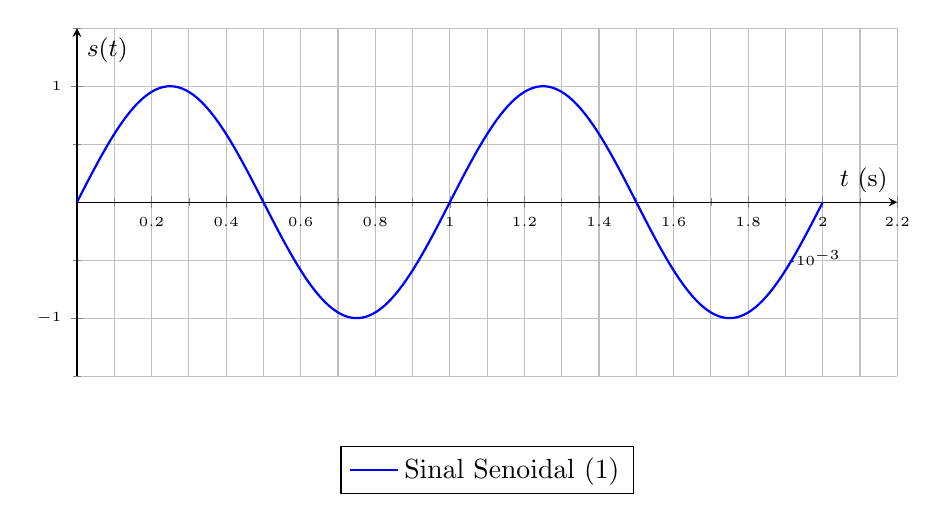
\begin{tikzpicture}
\begin{axis}[
    width=12cm, height=6cm,     % Dimensões do gráfico
    axis lines = middle,        % Eixos cruzados no centro
    xlabel = {$t$ (s)},         % Rótulo do eixo X
    ylabel = {$s(t)$},          % Rótulo do eixo Y
    label style={font=\small},
    tick label style={font=\tiny},
    grid = both,                % Grade para facilitar a leitura de valores
    minor tick num = 1,
    domain = 0:0.002,           % Domínio (ex: 2ms para ver 2 ciclos de 1kHz)
    samples = 200,              % Suavidade da curva
    xmin=0, xmax=0.0022,
    ymin=-1.5, ymax=1.5,
    legend style={at={(0.5,-0.2)}, anchor=north, legend columns=-1}
]
    % Curva da Senoide: A * sin(2 * pi * f * x + fase)
    % Exemplo: Amplitude=1, Frequência=1000Hz (1kHz)
    \addplot [blue, thick] {1 * sin(deg(2 * pi * 1000 * x + 0))};
    \addlegendentry{Sinal Senoidal ($1\khz$)}

\end{axis}
\end{tikzpicture}
\end{center}